% v2v insertion snippets only; no manuscript source is included.
\begin{figure*}[t]
\centering
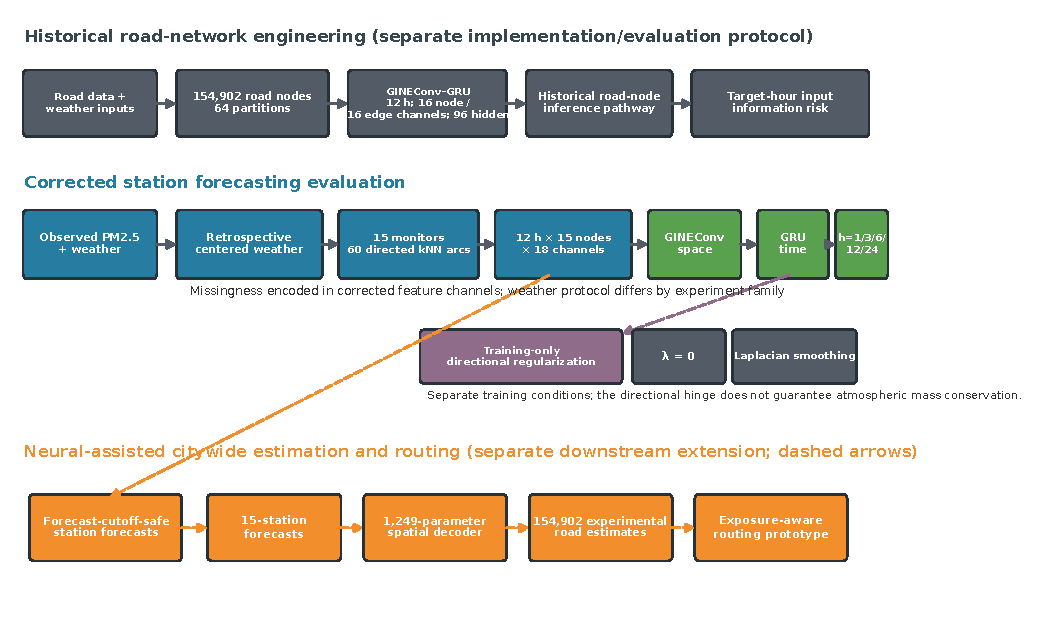
\includegraphics[width=\textwidth]{final_blr_results/ieee_publication_assets_v2v/figures/F01_architecture/F01_corrected_architecture.pdf}
\caption{The historical road-network lane documents a partitioned GINEConv–GRU implementation and its distinct input protocol; it is not the corrected station-graph benchmark. The corrected forecasting graph has 15 station nodes and 60 directed kNN edges, with a 12-hour window and 18 channels. Weather handling differs across retrospective centered-weather and forecast-cutoff-safe evaluations. The directional hinge is a training-only objective evaluated on predictions; λ=0 and Laplacian are separate conditions. Dashed arrows denote experimental downstream station-to-road decoding and routing. Road-node values are estimates, not observed concentrations; no mass-conservation guarantee is implied.}
\label{fig:f01-corrected-architecture}
\end{figure*}

\begin{figure*}[t]
\centering
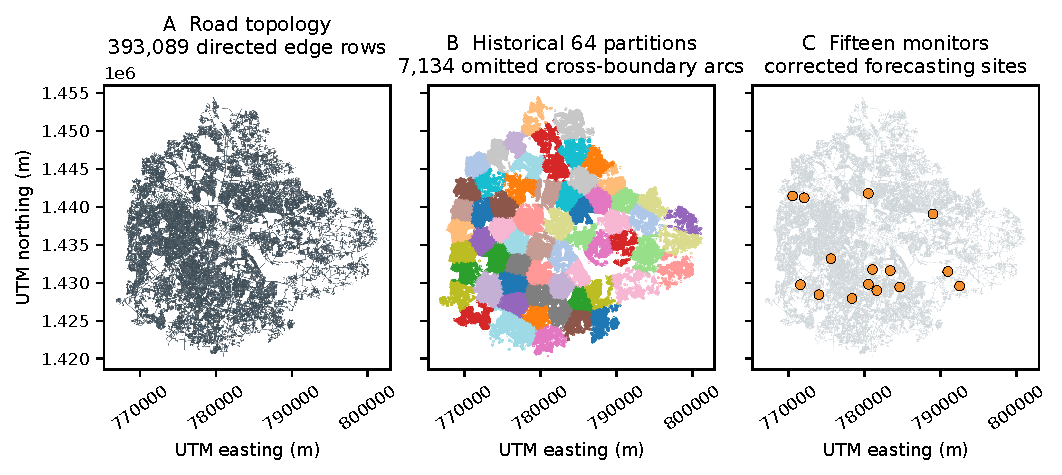
\includegraphics[width=\textwidth]{final_blr_results/ieee_publication_assets_v2v/figures/F02_graph_partitions/F02_bengaluru_graph.pdf}
\caption{Stored UTM graph and partition IDs; 154,902 nodes. The corrected forecasting model was evaluated on a separate 15-station, 60-edge kNN graph, not on the road graph. Arc and edge-row counts have different preprocessing semantics.}
\label{fig:f02-bengaluru-graph}
\end{figure*}

\begin{figure*}[t]
\centering
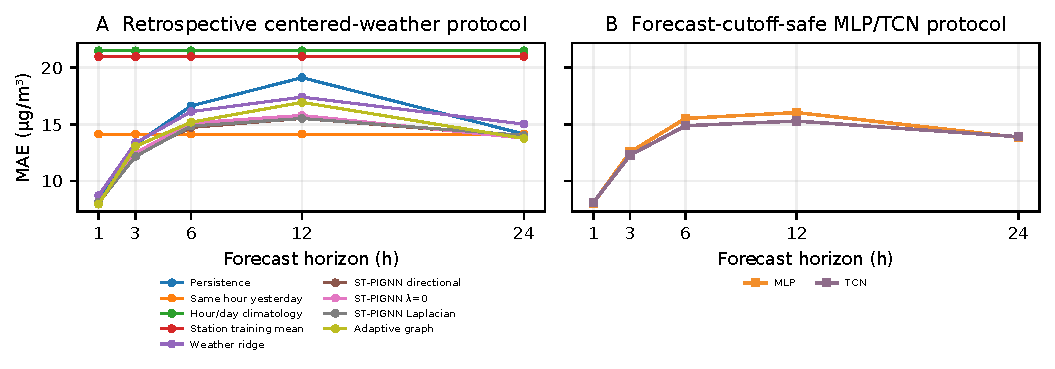
\includegraphics[width=\textwidth]{final_blr_results/ieee_publication_assets_v2v/figures/F03_forecasting_benchmarks/F03_multi_horizon_mae.pdf}
\caption{Five horizons and 14,583 saved pairs per horizon in the retrospective centered-weather panel; MLP/TCN use a separate forecast-cutoff-safe feature protocol. These are not identical-input architecture ablations. The full 17-variant inventory is provided separately; unfavorable results are retained.}
\label{fig:f03-multi-horizon-mae}
\end{figure*}

\begin{figure*}[t]
\centering
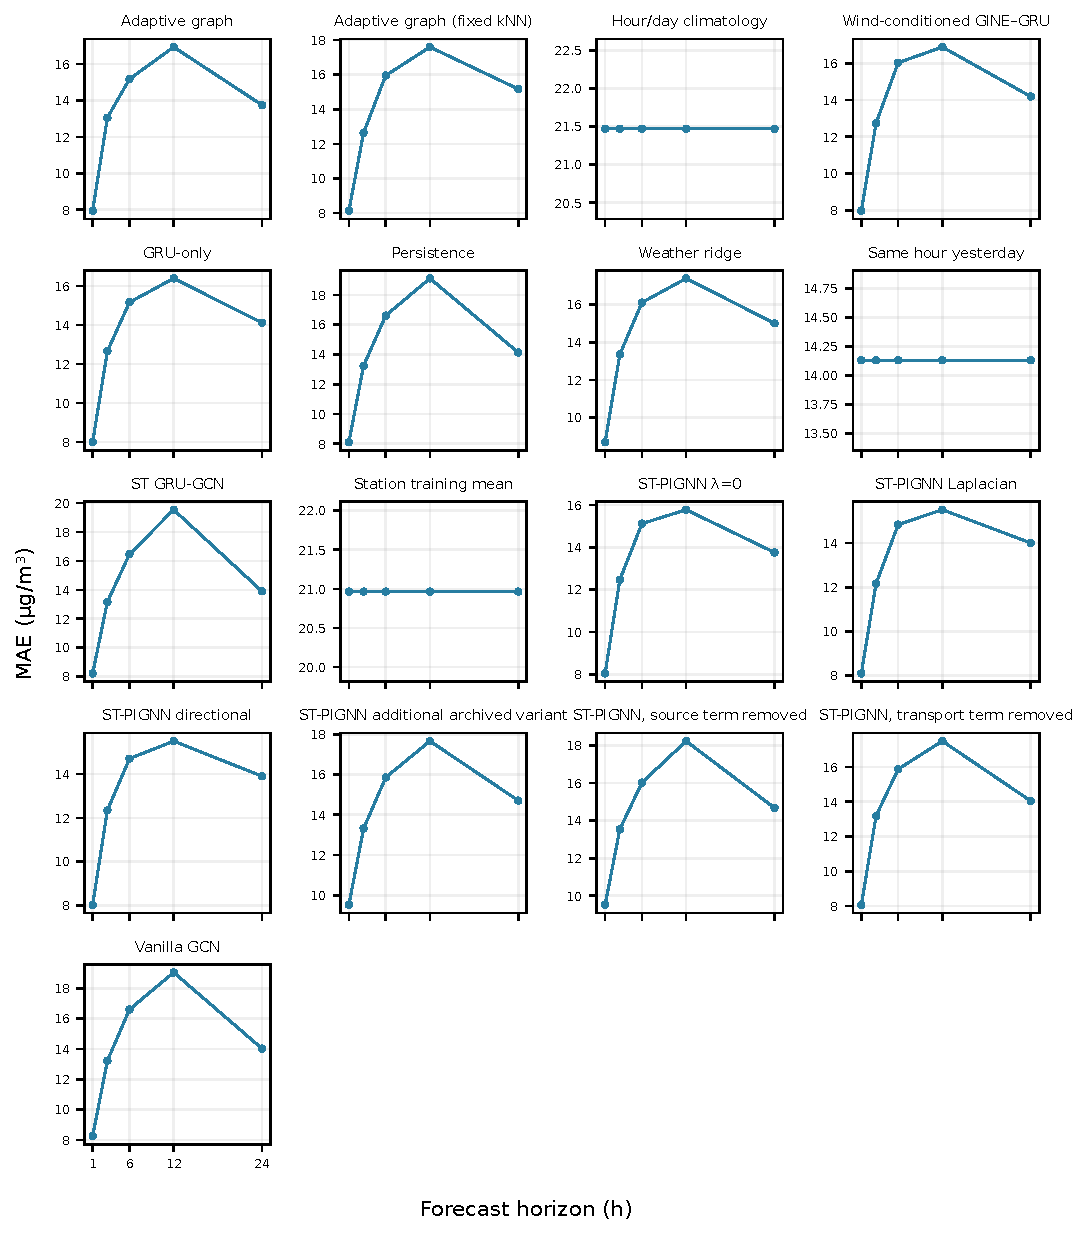
\includegraphics[width=\textwidth]{final_blr_results/ieee_publication_assets_v2v/figures/F03_forecasting_benchmarks/F03b_all_v2j_variants.pdf}
\caption{Small multiples show all 17 archived model variants separately at five horizons (14,583 pairs per horizon). All curves belong to the retrospective centered-weather station evaluation; variants are exploratory and share an exposed test period. MLP/TCN are not shown because their cutoff-safe protocol differs.}
\label{fig:f03b-all-v2j-variants}
\end{figure*}

\begin{figure*}[t]
\centering
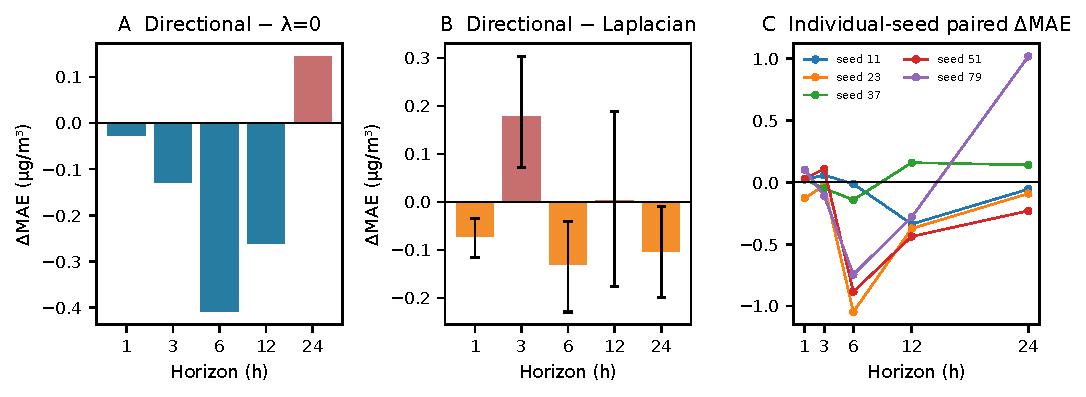
\includegraphics[width=\textwidth]{final_blr_results/ieee_publication_assets_v2v/figures/F04_physics_ablations/F04_directional_ablation.pdf}
\caption{Negative ΔMAE favors directional regularization. Panels A/B are five-seed ensemble differences; C shows individual-seed paired differences. No physical-specificity or mass-conservation inference follows. Multiplicity and seven-day block sensitivity are reported in T03.}
\label{fig:f04-directional-ablation}
\end{figure*}

\begin{figure*}[t]
\centering
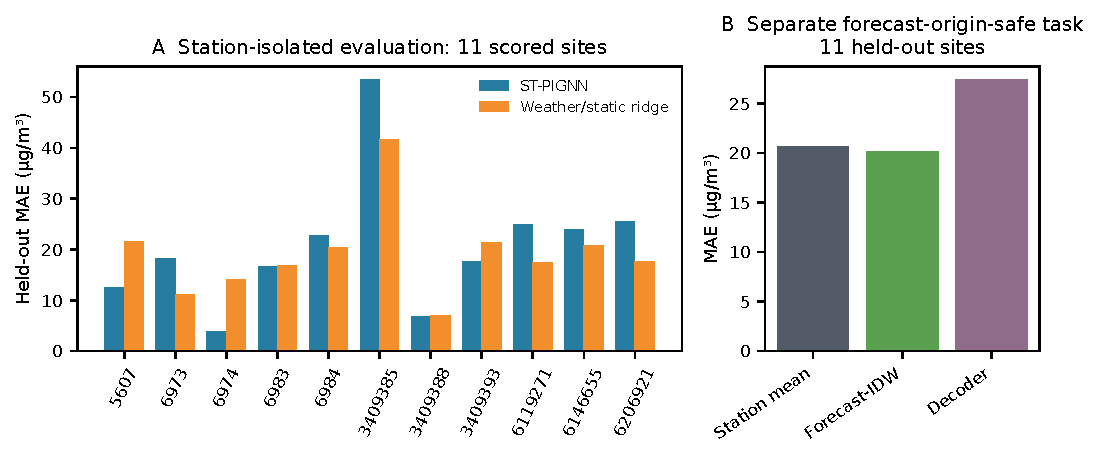
\includegraphics[width=\textwidth]{final_blr_results/ieee_publication_assets_v2v/figures/F05_spatial_validation/F05_spatial_holdouts.pdf}
\caption{Station-isolated evaluation uses 11 scored sites (four eligible stations had no test targets). Pooled observation-weighted MAE is ST-PIGNN 22.314 versus weather/static ridge 20.624 µg/m³; equal-site mean paired difference is +1.487 µg/m³ (station-bootstrap 95\% CI -2.577 to +5.328; 11 sites). Five sites favor ST-PIGNN and six favor ridge. Site 3409385 is influential. Separate six-hour decoder evaluation has pooled MAE 27.360 versus forecast-IDW 20.154; pooled and equal-site differences are distinct estimands. Repeated timestamps are not independent spatial sites.}
\label{fig:f05-spatial-holdouts}
\end{figure*}

\begin{figure*}[t]
\centering
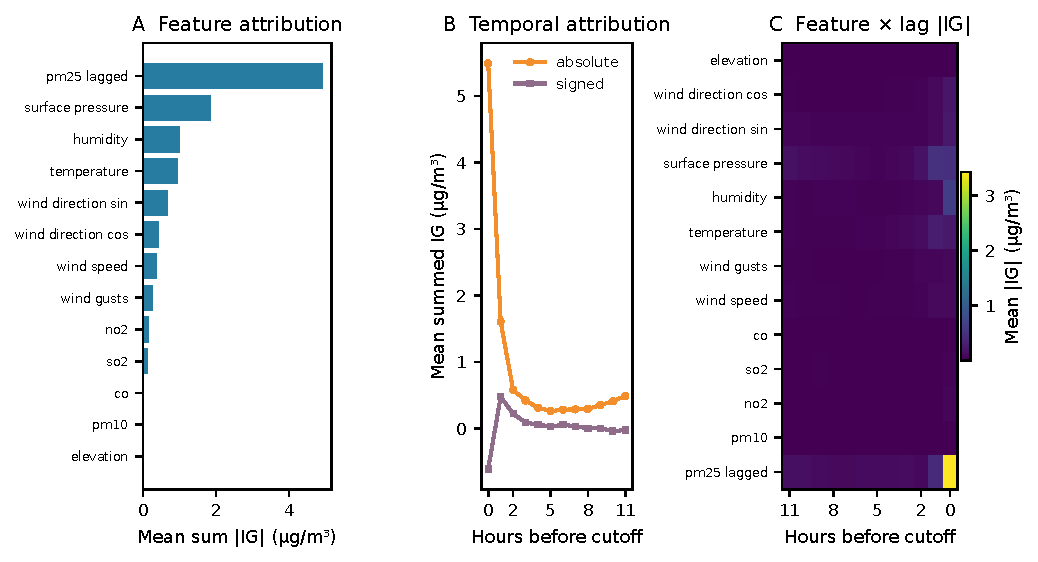
\includegraphics[width=\textwidth]{final_blr_results/ieee_publication_assets_v2v/figures/F06_captum_explainability/F06a_v2c_h1.pdf}
\caption{Real saved attribution tensors, primary training-mean baseline, 45 attributed records, 12 input hours. Mean absolute and signed IG are separate. Maximum completeness |delta| 2.1e-05 µg/m³; wrapper error 4.6e-05 µg/m³. IG is baseline-relative sensitivity, not causality or physics proof. Integration-step count is documented in source methodology.}
\label{fig:f06a-v2c-h1}
\end{figure*}

\begin{figure*}[t]
\centering
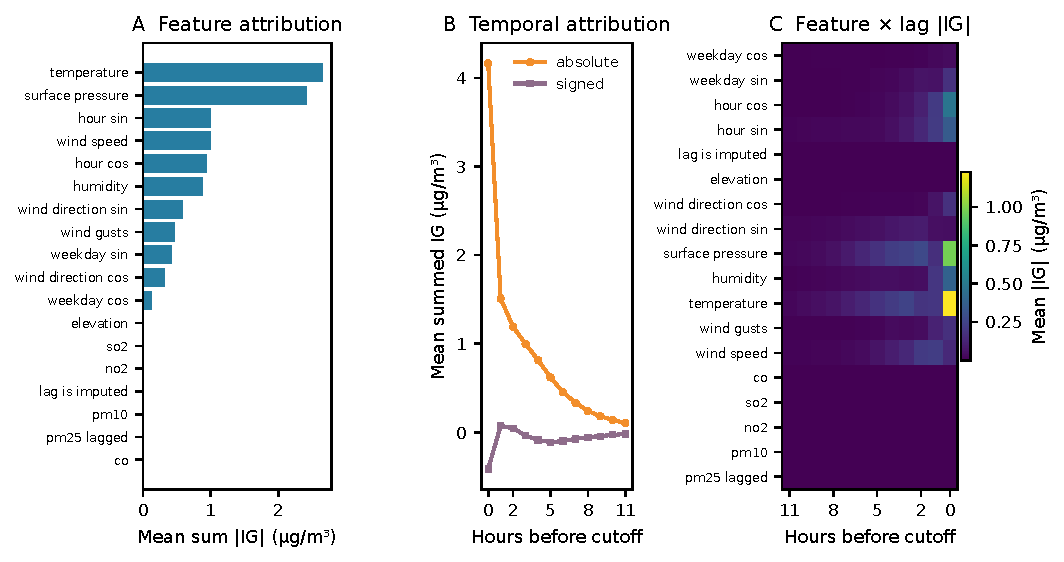
\includegraphics[width=\textwidth]{final_blr_results/ieee_publication_assets_v2v/figures/F06_captum_explainability/F06b_v2r_h6.pdf}
\caption{Real saved attribution tensors, primary training-mean baseline, 9 attributed records, 12 input hours. Mean absolute and signed IG are separate. Maximum completeness |delta| 7.8e-06 µg/m³; wrapper error 7.6e-06 µg/m³. IG is baseline-relative sensitivity, not causality or physics proof. Integration-step count is documented in source methodology.}
\label{fig:f06b-v2r-h6}
\end{figure*}

\begin{figure*}[t]
\centering
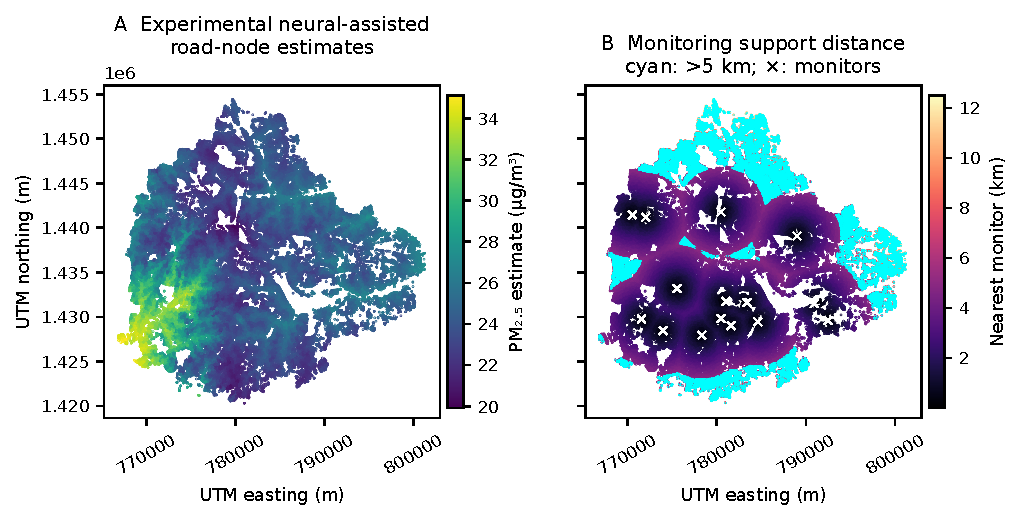
\includegraphics[width=\textwidth]{final_blr_results/ieee_publication_assets_v2v/figures/F07_citywide_estimation/F07_citywide_snapshot.pdf}
\caption{Earliest frozen origin, 2025-10-08 07:00 UTC, six-hour forecast; 154,902 saved node values without added smoothing. Station forecaster uses 15-station graph; road values use separate 1,249-parameter decoder. Decoder underperformed simple spatial controls; roadside accuracy is unvalidated. 19.45\% of nodes lie >5 km from a monitor; 60.58\% are outside the monitor convex hull.}
\label{fig:f07-citywide-snapshot}
\end{figure*}

\begin{figure*}[t]
\centering
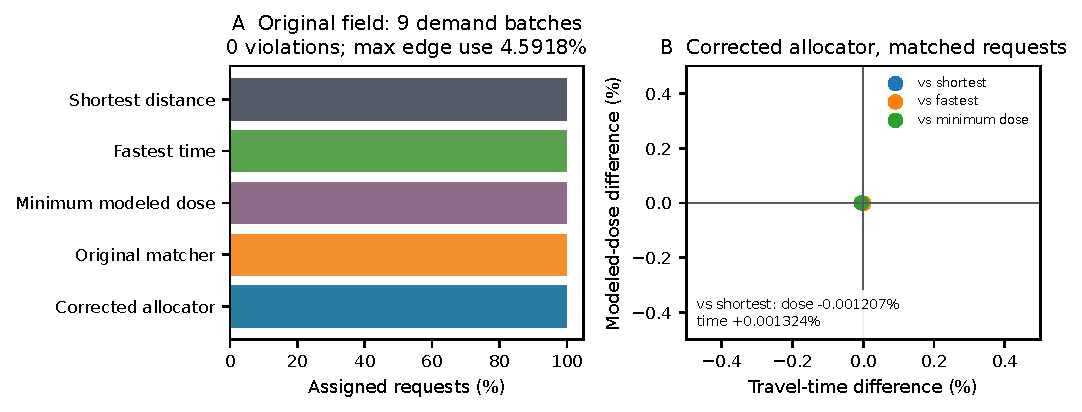
\includegraphics[width=\textwidth]{final_blr_results/ieee_publication_assets_v2v/figures/F08_routing_evaluation/F08_routing_tradeoff.pdf}
\caption{Original concentration scenario; nine frozen demand batches (252 requests per method). Maximum edge utilization in this scenario was 4.5918\% (seed 37, demand 48); the 5.4054\% maximum belongs to the spatial-sine perturbation across all four saved concentration fields. Corrected allocator and original matcher assigned all low-load requests; zero shared-edge violations. Corrected versus shortest: −0.001207\% modeled dose and +0.001324\% travel time. Axes span ±0.5\% to show the small differences. This is modeled dose, not measured exposure reduction or classical matching stability.}
\label{fig:f08-routing-tradeoff}
\end{figure*}

\begin{figure*}[t]
\centering
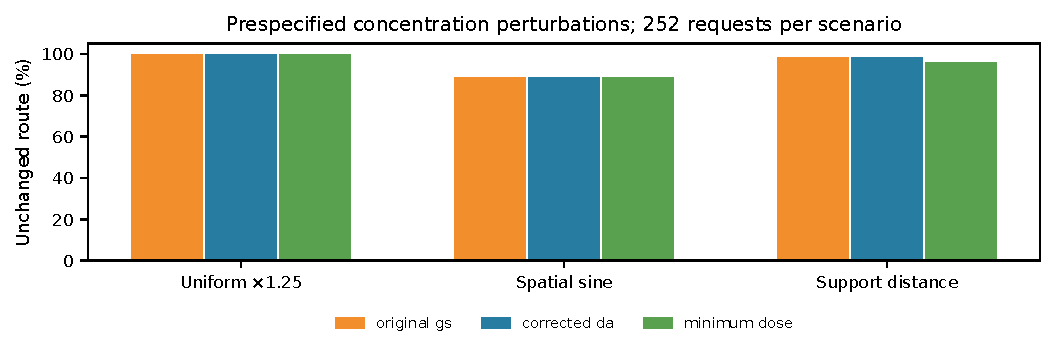
\includegraphics[width=\textwidth]{final_blr_results/ieee_publication_assets_v2v/figures/F08_routing_evaluation/F08b_routing_sensitivity.pdf}
\caption{The saved routing study contains four fields: one original concentration field plus three prespecified perturbations (uniform scaling, spatial sine, and support-distance perturbation). Each perturbation has 252 requests. Bars show route identity stability, not calibrated exposure uncertainty. Assignment stability was 100\% and declared edge-capacity violations zero in these low-load scenarios. No measured human exposure validation.}
\label{fig:f08b-routing-sensitivity}
\end{figure*}
